
\section{Convergence Analysis}\label{sec:conv}
In this section we analyze the convergence rate of \texttt{SimpleSolver} algorithm. In other words, we investigate whether this algorithm can converge to the optimal solution after finite iterations or not. For this purpose, we should show that after finite iterations, the algorithm's solution approach to the optimal solution with ratio $\epsilon$ or mathematically, the following equation should be satisfied. \\
For $\forall ~~ 0<\epsilon<1, \exists ~ i$ that the Equation \ref{eq:convergence} is satisfied.
\begin{equation}
    \label{eq:convergence}
    \| X_i -X^* \|_2 \leq \epsilon \|X_0 - X^* \|_2
\end{equation}
where $X_i$ and $X_0$ are the algorithm's solution in the $i$-th and first iterations, respectively. $\epsilon$ is lower than 1, but our desired value is very close to zero like 0.001 or $10^{-5}$. When we can find an $i$ such that the Equation \ref{eq:convergence} is established in that iteration, then we can conclude the algorithm can converge to the optimal solution with ratio $\epsilon$.
Theorem \ref{thrm:convergence} is equivalent to Equation \ref{eq:convergence} in the context of \texttt{SimpleSolver} algorithm.

\begin{theorem}
    Each iteration $i$ of \texttt{SimpleSolver} computes feasible $\overrightarrow{f}_i \in \mathds{R}^E$ such that
    \begin{center}
        $\mathds{E}[\xi_r(\overrightarrow{f}_i)]-\xi_r(\overrightarrow{f}_{opt}) \leq (1-\frac{1}{\tau})^i (\xi_r(\overrightarrow{f}_0) - \xi_r(\overrightarrow{f}_{opt}))$ 
    \end{center}
    \label{thrm:convergence}
\end{theorem}
where $\xi_r(\overrightarrow{f}_i)$, $\xi_r(\overrightarrow{f}_{opt})$, and $\xi_r(\overrightarrow{f}_0)$ are the energy of $i$-th iteration, optimal energy, and energy of primary current flow, respectively. $\tau$ is the condition number of spanning tree of $T$ which is fixed in all iterations and it is positive. Therefore, $(1-\frac{1}{\tau})$ would be lower than 1 and as $i$ grows, the value of $(1-\frac{1}{\tau})^i$ becomes closer to zero. The proof of Theorem \ref{thrm:convergence} is divided into three steps. In Section \ref{cycle-update-progress}, we analyze the energy gain of a single algorithm iteration, in Section \ref{distance-to-optimality}, we bound the distance to optimality in a single algorithm iteration, and in Section \ref{section:convergence-proof}, we connect these to prove the theorem.

\subsection{Cycle Update Progress}
\label{cycle-update-progress}
In Section \ref{algorith:cycle-update}, we observed that the current flow vector in each iteration is updated with 

$-\frac{\Delta_{c_e}(\overrightarrow{f}_i)}{R_e} \overrightarrow{c}_e$ vector, where $\Delta_{c_e}(\overrightarrow{f}_i) = \overrightarrow{f}_i^\top \mathbf{R} \overrightarrow{c}_e$ and $R_e=\overrightarrow{c}_e^\top \mathbf{R} \overrightarrow{c}_e$. In this section, from a mathematical perspective, we investigate why this update vector approaches the algorithm to the optimal solution.\\
The first idea that comes to our mind when we want to calculate the optimal update value is derivation. Therefore, we consider the $\xi_r(\overrightarrow{f}+\alpha \overrightarrow{c})$ and find the best $\alpha$ that can minimize the energy.
\begin{center}
    
    $\frac{\partial \xi_r(\overrightarrow{f}+\alpha \overrightarrow{c})}{\partial \alpha} =
    \frac{\partial (\overrightarrow{f}+\alpha \overrightarrow{c})^\top \textbf{R} (\overrightarrow{f}+\alpha \overrightarrow{c})}{\partial \alpha}= 2 \overrightarrow{f} \textbf{R} \overrightarrow{c} + 2 \alpha \overrightarrow{c}^\top \textbf{R} \overrightarrow{c}$
\end{center}
\begin{equation}
    \label{gradient-to-alpha}
    2 \overrightarrow{f} \textbf{R} \overrightarrow{c} + 2 \alpha \overrightarrow{c}^\top \textbf{R} \overrightarrow{c}=0 \implies \alpha^* = -\frac{\overrightarrow{f} \textbf{R} \overrightarrow{c}}{\overrightarrow{c}^\top \textbf{R} \overrightarrow{c}}
\end{equation}
In the second stage, we verify whether this $\alpha^*$ can decrease the energy of the electrical network in each iteration or not. Therefore, we calculate the energy difference between two sequential iterations by substitution of $\alpha^*$. 
\begin{center}
    $\xi_r(\overrightarrow{f}+\alpha^* \overrightarrow{c}) - \xi_r(\overrightarrow{f})=(\overrightarrow{f}+\alpha^* \overrightarrow{c})^\top \textbf{R} (\overrightarrow{f}+\alpha^* \overrightarrow{c}) - \overrightarrow{f}^\top \textbf{R} \overrightarrow{f}=$
\end{center}
\begin{equation}
\label{energy-decrease}
    {\alpha^*}^2 \overrightarrow{c} \textbf{R} \overrightarrow{c}+2 \alpha^* \overrightarrow{f}^\top \textbf{R} \overrightarrow{c}=-\frac{(\overrightarrow{f}^\top \mathbf{R} \overrightarrow{c})^2}{\overrightarrow{c}^\top \mathbf{R} \overrightarrow{c}}
\end{equation}
According to Equation \ref{energy-decrease}, it can be seen the energy in two sequential iterations decreases if we update the flow vector with the corresponding $\alpha$.
We summarize the update value and energy decrease in Lemma \ref{energy-improvement}.
\begin{lemma}
    \label{energy-improvement}
    For $\overrightarrow{f} \in \mathds{R}^E$, $\overrightarrow{c} \in \mathds{R}^E$, and $\alpha^*=-\frac{\overrightarrow{f} \mathbf{R} \overrightarrow{c}}{\overrightarrow{c}^\top \mathbf{R} \overrightarrow{c}} \in \mathds{R}$ we have
    \begin{center}
        $argmin_{\alpha \in \mathds{R}}~ \xi_r(\overrightarrow{f}+\alpha \overrightarrow{c})=-\frac{\overrightarrow{f} \mathbf{R} \overrightarrow{c}}{\overrightarrow{c}^\top \mathbf{R} \overrightarrow{c}} \text{~~~~~ and ~~~~~}\xi_r(\overrightarrow{f}+\alpha^* \overrightarrow{c}) - \xi_r(\overrightarrow{f})=-\frac{(\overrightarrow{f}^\top \mathbf{R} \overrightarrow{c})^2}{\overrightarrow{c}^\top \mathbf{R} \overrightarrow{c}}$
    \end{center}
\end{lemma}
If we define $\overrightarrow{c}=\overrightarrow{c}_e$ is a tree cycle for some off-tree edge $e \in E \setminus T$, since $R_e= \overrightarrow{c}_e^\top \mathbf{R} \overrightarrow{c}_e$ and $\Delta_{c_e}(\overrightarrow{f})=\overrightarrow{f}^\top \mathbf{R} \overrightarrow{c}_e$, this procedure is precisely the iterative step of \texttt{SimpleSolver}, i.e. a cycle update. Lemma \ref{lemma:cycle-update} states the energy decrease of a cycle update is exactly the energy of a resistor with resistance $R_e$ and potential drop $\Delta_{c_e}(\overrightarrow{f})$.
\begin{lemma}
    \label{lemma:cycle-update}
    For feasible $\overrightarrow{f} \in \mathds{R}^E$ and $e \in E \setminus T$ we have
    \begin{center}
        $\xi_r(\overrightarrow{f}-\frac{\Delta_{c_e}(\overrightarrow{f})}{R_e} \overrightarrow{c}_e) - \xi_r(\overrightarrow{f})=-\frac{\Delta_{c_e}(\overrightarrow{f})^2}{R_e}$
    \end{center}
\end{lemma}

\subsection{Distance to Optimality}
\label{distance-to-optimality}
In this section, we calculate the gap between $\overrightarrow{f}$ and $\overrightarrow{v}$ in the dual problem. Since the energy function of $\overrightarrow{f}$ is convex and Slater's condition is satisfied, the duality gap between the primal and dual problems is zero. Figure \ref{fig:duality-gap} shows the gap between the primal and dual problems. 
\begin{center}
\begin{figure}[!ht]
\begin{tikzpicture}
    \node[anchor=south west,inner sep=0] at (5.0,0.0) {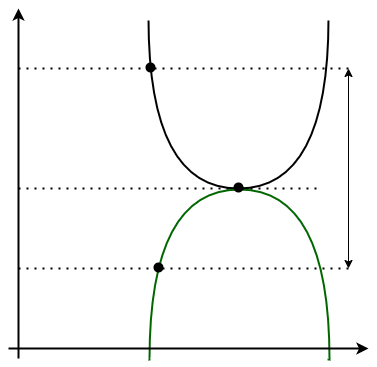
\includegraphics[scale=0.5]{Images/Convergence/dual_problem.drawio.png}};
    \draw (4.8,1.5) node {$\xi_r(\overrightarrow{v}_i)$};
    \draw (7.1,0.7) node {$\xi_r(\overrightarrow{v})$};
    \draw (7.1,5.9) node {$\xi_r(\overrightarrow{f})$};
    \draw (4.8,5.5) node {$\xi_r(\overrightarrow{f}_i)$};
    \draw (3.5,3.2) node {$\xi_r(\overrightarrow{f}_{opt})=\xi_r(\overrightarrow{v}_{opt})$};
    \draw (12.2,3.4) node {$gap(\overrightarrow{f}_i, \overrightarrow{v}_i)$};
\end{tikzpicture}
\caption{Visualization for primal and dual functions in electrical network energy} 
\label{fig:duality-gap}
\end{figure}
\end{center}
Figure \ref{fig:duality-gap} makes smoother understanding the distance between $\overrightarrow{f}$, $\overrightarrow{f}_{opt}$, $\overrightarrow{v}$, and $\overrightarrow{v}_{opt}$. Here we derive a simple expression for the duality gap between $\overrightarrow{f}$ and its tree-induced voltages $\overrightarrow{v}$ in terms of cycle potentials. Lemma \ref{lemma:tree-gap} states this quantity in terms of cycle potentials.
\begin{lemma}
    \label{lemma:tree-gap}
    For feasible $\overrightarrow{f} \in \mathds{R}^E$ and tree induced voltages $\overrightarrow{v} \in \mathds{R}^V$ we have
    \begin{center}
        $gap(\overrightarrow{f},\overrightarrow{v})=\sum_{e \in E \setminus T} \frac{\Delta_{c_e}(\overrightarrow{f})^2}{r_e}$
    \end{center}
\end{lemma}
\textit{Proof.} We defined the primal and dual energy in Section \ref{section:electrical-flow-duality}, therefore, we have
\begin{equation}
    \label{eq:gap-definition}
    gap(\overrightarrow{f},\overrightarrow{v})=\overrightarrow{f}^\top \mathbf{R} \overrightarrow{f} - (2 \overrightarrow{v}^\top \overrightarrow{\chi} - \overrightarrow{v}^\top \mathbf{L} \overrightarrow{v})
\end{equation}
If we substitute $\mathbf{B}^\top \overrightarrow{f} = \overrightarrow{\chi}$ and $\mathbf{L}=\mathbf{B}^\top \mathbf{R}^{-1} \mathbf{B}$ in Equation \ref{eq:gap-definition}, we get
\begin{center}
    $gap(\overrightarrow{f},\overrightarrow{v})=\overrightarrow{f}^\top \mathbf{R} \overrightarrow{f} - 2 \overrightarrow{v}^\top \mathbf{B}^\top \overrightarrow{f} + \overrightarrow{v}^\top \mathbf{B}^\top \mathbf{R}^{-1} \mathbf{B} \overrightarrow{v})=(\mathbf{R}\overrightarrow{f}-\mathbf{B}\overrightarrow{v})^\top \mathbf{R}^{-1} (\mathbf{R}\overrightarrow{f}-\mathbf{B}\overrightarrow{v})$
\end{center}
\begin{equation}
    =\sum_{e \in E } \frac{1}{r_e}(\overrightarrow{f}(e)r_e - \Delta_{\overrightarrow{v}}(e))^2
\end{equation}
In this stage, we used the definition of tree voltages in Equation \ref{eq:tree-voltages} to simplify $gap(\overrightarrow{f}, \overrightarrow{v})$.
\begin{equation}
    \label{eq:tree-voltages}
    \forall~ a,b \in V ~~:~~ \Delta_{\overrightarrow{v}}(a,b)=\overrightarrow{v}(a) - \overrightarrow{v} (b) = \sum_{e \in P_{as}} \overrightarrow{f}(e) r_e + \sum_{e \in P_{sb}} \overrightarrow{f}(e) r_e = \sum_{e \in P_{ab}} \overrightarrow{f}(e) r_e
\end{equation}
We know that 
\begin{equation}
    \label{eq:tree-voltages-cases}
    \overrightarrow{f}(e) r_e - \Delta_{\overrightarrow{v}}(e) = \begin{cases}
        0 &  \forall ~ e \in T \\
        \Delta_{c_e}(\overrightarrow{f})  &  \forall ~ e \in E \setminus T 
\end{cases}
\end{equation}
is satisfied during the algorithm. Figure \ref{fig:voltage-difference} shows an electrical network to smooth understanding of Equation \ref{eq:tree-voltages-cases}.
\begin{figure}[!h]
    \centering
    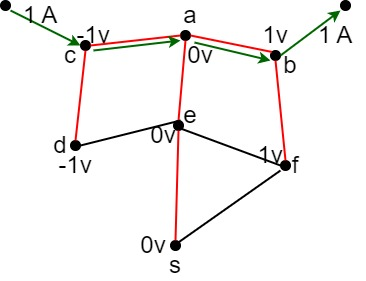
\includegraphics[scale=0.44]{Images/Convergence/voltage_difference.jpg}
    \caption{An example of an electrical network with induced current 1A between nodes $b$ and $c$ (the resistance of all edges is equal to $1 \Omega$)}
    \label{fig:voltage-difference}
\end{figure} \\
1A current is induced between nodes $b$ and $c$ in the electrical network in Figure \ref{fig:voltage-difference}. Assume one edge from the spanning tree, which is shown with red edges in the graph, like edge $(c,a)$, and investigate the relation $\overrightarrow{f}(e)r_e - \Delta_{\overrightarrow{v}}(e)$ in it (the resistance of all edges in the network is equal to $1 \Omega$)). 
\begin{center}
    $\overrightarrow{f}((c,a))r_{(c,a)} = (1 A) \times (1 \Omega)=1v$\\
    ~\\
    $\Delta_{\overrightarrow{v}}(c,a)=\overrightarrow{v}(c) - \overrightarrow{v} (a) = \sum_{e \in P_{cs}} \overrightarrow{f}(e) r_e + \sum_{e \in P_{sa}} \overrightarrow{f}(e) r_e $\\
    $= [\overrightarrow{f}((e,s))r_{(e,s)} + \overrightarrow{f}((a,e))r_{(a,e)} + \overrightarrow{f}((c,a))r_{(c,a)}]-[\overrightarrow{f}((e,s))r_{(e,s)} + \overrightarrow{f}((a,e))r_{(a,e)}]$\\
    $=\overrightarrow{f}((c,a))r_{(c,a)}=(1 A) \times (1 \Omega)=1v$\\
    ~\\
    $\implies \overrightarrow{f}((c,a))r_{(c,a)} - \Delta_{\overrightarrow{v}}(c,a)=0$
\end{center}
Now, consider an edge outside of the spanning tree such as $(e,f)$ and investigate the relation $\overrightarrow{f}(e)r_e - \Delta_{\overrightarrow{v}}(e)$ for this edge.
\begin{center}
    $\overrightarrow{f}((e,f))r_{(e,f)} = (0 A) \times (1 \Omega)=0v$\\
    ~\\
    $\Delta_{\overrightarrow{v}}(e,f)=\overrightarrow{v}(e) - \overrightarrow{v} (f) = \sum_{e \in P_{es}} \overrightarrow{f}(e) r_e + \sum_{e \in P_{sf}} \overrightarrow{f}(e) r_e $\\
    $= [\overrightarrow{f}((e,s))r_{(e,s)}]-[\overrightarrow{f}((e,s))r_{(e,s)} + \overrightarrow{f}((a,e))r_{(a,e)} + \overrightarrow{f}((b,a))r_{(b,a)}+ \overrightarrow{f}((f,b))r_{(f,b)}]$\\
    $=-\overrightarrow{f}((a,e))r_{(a,e)} - \overrightarrow{f}((b,a))r_{(b,a)} - \overrightarrow{f}((f,b))r_{(f,b)}$\\
    $=-(0 A) \times (1 \Omega) -(1 A) \times (1 \Omega) -(0 A) \times (1 \Omega)=-1v$\\
    ~\\
    $\implies \overrightarrow{f}((e,f))r_{(e,f)} - \Delta_{\overrightarrow{v}}(e,f)=$\\
    $\overrightarrow{f}((a,e))r_{(a,e)} + \overrightarrow{f}((b,a))r_{(b,a)} + \overrightarrow{f}((f,b))r_{(f,b)}$\\
    $=\sum{e \in P_{ef}}\overrightarrow{f}(e)r_e=\Delta_{c_{(e,f)}}(\overrightarrow{f})$
\end{center}
We showed the correctness of Equation \ref{eq:tree-voltages-cases} with an electrical network example. Therefore, if we substitute Equation \ref{eq:tree-voltages-cases} in the simplified definition of $gap(\overrightarrow{f}, \overrightarrow{v})$
\begin{center}
    $gap(\overrightarrow{f}, \overrightarrow{v})=\sum_{e \in E } \frac{1}{r_e}(\overrightarrow{f}(e)r_e - \Delta_{\overrightarrow{v}}(e))^2$\\
    $=\sum_{e \in T } \frac{1}{r_e}(\overrightarrow{f}(e)r_e - \Delta_{\overrightarrow{v}}(e))^2 + \sum_{e \in E \setminus T } \frac{1}{r_e}(\overrightarrow{f}(e)r_e - \Delta_{\overrightarrow{v}}(e))^2$\\
    $=0+\sum_{e \in E \setminus T} \frac{1}{r_e}\Delta_{c_e}(\overrightarrow{f})^2=\sum_{e \in E \setminus T} \frac{1}{r_e}\Delta_{c_e}(\overrightarrow{f})^2$
\end{center}
The proof in this step is complete and Lemma \ref{lemma:tree-gap} is proved for each electrical network. $\square$

\subsection{Convergence Proof}
\label{section:convergence-proof}
In this section, we find an interpretation of energy decrease in two sequential iterations according to the duality gap in order to bound the convergence of \texttt{SimpleSolver} algorithm.\\
In the first step, we state the expectation of energy decrease in two sequential iterations in Lemma \ref{lemma:expected-progress}.
\begin{lemma}
    \label{lemma:expected-progress}
    For iteration $i$ of \texttt{SimpleSolver} algorithm, we have
    \begin{center}
    $\mathds{E}[\xi_r(\overrightarrow{f}_i)-\xi_r(\overrightarrow{f}_{i-1})|~gap(\overrightarrow{f}_{i-1}, \overrightarrow{v}_{i-1})]=-\frac{gap(\overrightarrow{f}_{i-1}, \overrightarrow{v}_{i-1})}{\tau}$
    \end{center}
\end{lemma}
\textit{Proof.} In each iteration $i$, \texttt{SimpleSolver} algorithm picks a random $e_i \in E \setminus T$ with probability $p_{e_i}$. Therefore, we can calculate the expectation as follows.
\begin{equation}
    \label{eq:energy-decrease-expectation}
    \mathds{E}[\xi_r(\overrightarrow{f}_i)-\xi_r(\overrightarrow{f}_{i-1})|~gap(\overrightarrow{f}_{i-1}, \overrightarrow{v}_{i-1})]=\sum_{e \in E} p_e [\xi_r(\overrightarrow{f}_i)-\xi_r(\overrightarrow{f}_{i-1})]
\end{equation}
According to the \texttt{SimpleSolver} algorithm, $p_e=\frac{1}{\tau}\frac{R_e}{r_e}$ and using Lemma \ref{lemma:cycle-update}, the energy decreas between two sequential iterations for $\forall~e \in E \setminus T$ is equal to $-\frac{\Delta_{c_e}(\overrightarrow{f})^2}{R_e}$ and it is zero for edges on spanning tree. By substitution of these quantities in Equation \ref{eq:energy-decrease-expectation}, we get
\begin{center}
    
    $\mathds{E}[\xi_r(\overrightarrow{f}_i)-\xi_r(\overrightarrow{f}_{i-1})|~gap(\overrightarrow{f}_{i-1}, \overrightarrow{v}_{i-1})]=\sum_{e \in E} p_e [\xi_r(\overrightarrow{f}_i)-\xi_r(\overrightarrow{f}_{i-1})]$
\end{center}
\begin{equation}
    \label{eq:simplified-energy-decrease-expectation}
    =\sum_{e \in E\setminus T} \frac{1}{\tau}\frac{R_e}{r_e} (-\frac{\Delta_{c_e}(\overrightarrow{f}_{i-1})^2}{R_e})
\end{equation}
In Lemma \ref{lemma:tree-gap}, we observed that $\sum_{e \in E \setminus T} \frac{\Delta_{c_e}(\overrightarrow{f})^2}{r_e}=gap(\overrightarrow{f},\overrightarrow{v})$. By using Lemma \ref{lemma:tree-gap}, Equation \ref{eq:simplified-energy-decrease-expectation} can be simplified as follows.
\begin{center}
    $\mathds{E}[\xi_r(\overrightarrow{f}_i)-\xi_r(\overrightarrow{f}_{i-1})|~gap(\overrightarrow{f}_{i-1}, \overrightarrow{v}_{i-1})]=\sum_{e \in E\setminus T} \frac{1}{\tau}\frac{R_e}{r_e} (-\frac{\Delta_{c_e}(\overrightarrow{f}_{i-1})^2}{R_e})$\\
    $=-\frac{1}{\tau} \sum_{e \in E\setminus T} \frac{\Delta_{c_e}(\overrightarrow{f}_{i-1})^2}{r_e})=-\frac{gap(\overrightarrow{f}_{i-1}, \overrightarrow{v}_{i-1})}{\tau}$
\end{center}
Hence, the proof of Lemma \ref{lemma:expected-progress} is finished. $\square$ \\
Next, we try to show that each iteration decreases the expected energy difference between the current flow and the optimal flow by a ratio $(1-\frac{1}{\tau})$. Lemma \ref{lemma:convergence-rate} expresses this.
\begin{lemma}
    \label{lemma:convergence-rate}
    For all $i \geq 0$, we define a random variable $D_i \stackrel{\text{def}}{=} \xi_r(\overrightarrow{f}_i)-\xi_r(\overrightarrow{f}_{opt})$. Then for all iterations $i \geq 1$, we have
    \begin{center}
        $\mathds{E}[D_i] \leq (1-\frac{1}{\tau}) \mathds{E}[D_{i-1}]$
    \end{center}
\end{lemma}
\textit{Proof.} Since in each iteration of \texttt{SimpleSolver}, one of a finite number of edges is chosen, clearly, $D_i$ is a discrete random variable and by the law of total expectation we have
\begin{equation}
    \label{eq:D-expectation}
    \mathds{E}[D_i]=\sum_{e} \mathds{E}[D_i|D_{i-1}=c]Pr[D_{i-1}=c]
\end{equation}
We try to simplify $\mathds{E}[D_i|D_{i-1}=c]$.
\begin{center}
    
    $\mathds{E}[D_i|D_{i-1}=c] = \mathds{E}[\xi_r(\overrightarrow{f}_i)-\xi_r(\overrightarrow{f}_{opt})|D_{i-1}=c]$\\
    $= \mathds{E}[(\xi_r(\overrightarrow{f}_i) - \xi_r(\overrightarrow{f}_{i-1}))+(\xi_r(\overrightarrow{f}_{i-1}) - \xi_r(\overrightarrow{f}_{opt}))|D_{i-1}=c] $\\
    $= \mathds{E}[(\xi_r(\overrightarrow{f}_i) - \xi_r(\overrightarrow{f}_{i-1}))+D_{i-1}|D_{i-1}=c] $
\end{center}
\begin{equation}
    \label{eq:conditional-expectation-D}
    = c + \mathds{E}[(\xi_r(\overrightarrow{f}_i) - \xi_r(\overrightarrow{f}_{i-1}))|D_{i-1}=c]
\end{equation}
From Figure \ref{fig:duality-gap}, it can be easily observed that $D_{i-1} \leq gap(\overrightarrow{f}_{i-1},\overrightarrow{v}_{i-1})$ is always satisfied. Using this fact and Lemma \ref{lemma:expected-progress}, we will have
\begin{equation}
    \label{eq:conditional-expectation-D-gap}
    \mathds{E}[(\xi_r(\overrightarrow{f}_i) - \xi_r(\overrightarrow{f}_{i-1}))|D_{i-1}=c]=-\frac{gap(\overrightarrow{f}_{i-1}, \overrightarrow{v}_{i-1})}{\tau} \leq -\frac{D_{i-1}}{\tau}=-\frac{c}{\tau}
\end{equation}
By substitution of Equation \ref{eq:conditional-expectation-D-gap} in Equation \ref{eq:conditional-expectation-D}, we can obtain that $\mathds{E}[D_i|D_{i-1}=c] \leq c -\frac{c}{\tau}$. Therefore, 
\begin{center}
    $\mathds{E}[D_i]=\sum_{e} \mathds{E}[D_i|D_{i-1}=c]Pr[D_{i-1}=c] \leq (1-\frac{1}{\tau})\sum_{e} c~Pr[D_{i-1}=c]=(1-\frac{1}{\tau})\mathds{E}[D_{i-1}]$.
\end{center}
\begin{flushright}
    $\square$
\end{flushright}
Finally, by induction on Lemma \ref{lemma:convergence-rate} and the definition of $D_i$ we can prove Theorem \ref{thrm:convergence} as the following.
\begin{center}
    $\mathds{E}[D_i] \leq (1-\frac{1}{\tau}) \mathds{E}[D_{i-1}] \leq (1-\frac{1}{\tau})^2 \mathds{E}[D_{i-2}] \leq \dots \leq (1-\frac{1}{\tau})^i \mathds{E}[D_{0}]$\\
    $\mathds{E}[\xi_r(\overrightarrow{f}_i)] - \xi_r(\overrightarrow{f}_{opt})=\mathds{E}[D_i] \leq (1-\frac{1}{\tau})^i \mathds{E}[D_{0}]=(1-\frac{1}{\tau})^i [\xi_r(\overrightarrow{f}_{0}) - \xi_r(\overrightarrow{f}_{opt})]$\\
    ~\\
    $\implies \mathds{E}[\xi_r(\overrightarrow{f}_i)] - \xi_r(\overrightarrow{f}_{opt}) \leq (1-\frac{1}{\tau})^i [\xi_r(\overrightarrow{f}_{0}) - \xi_r(\overrightarrow{f}_{opt})]$
\end{center}
As a result, we showed that \texttt{SimpleSolver} converges to the optimal solution after finite iterations.